\section{Analysis of type system}

\begin{figure}[htbp]
    \centerline{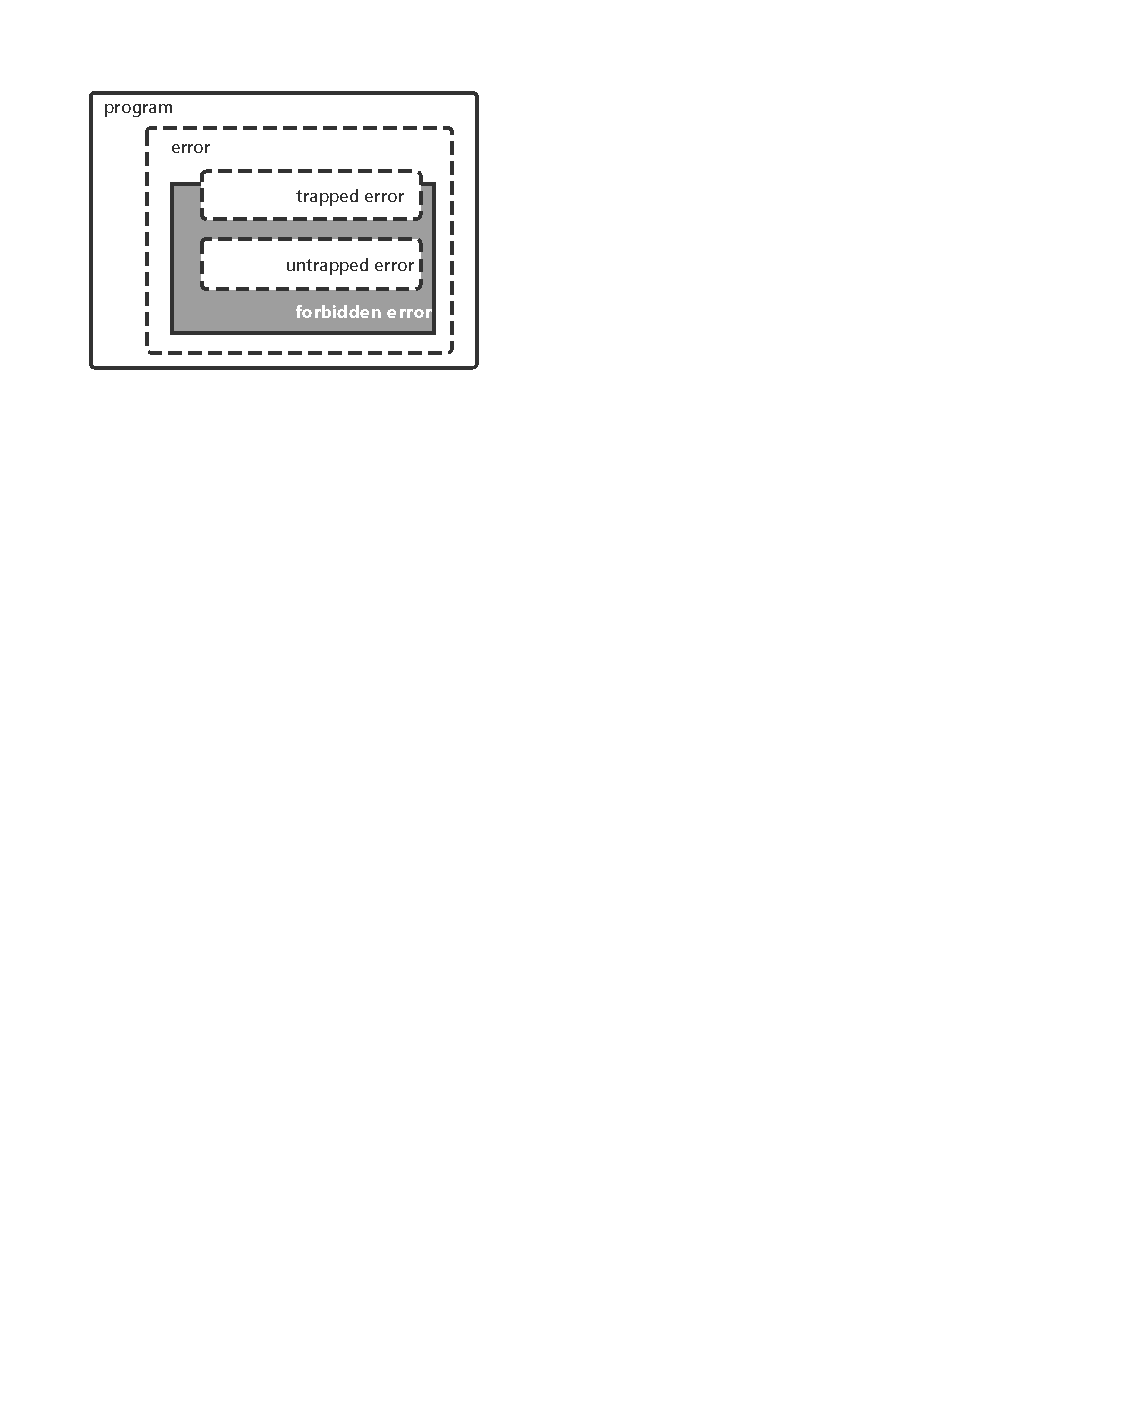
\includegraphics[scale=0.8]{figures/type-definition}}
    \caption{Definition of forbidden error}
    \label{fig:type-definition}
\end{figure}

The discussion here is based on L. Cardelli's definition of type systems.
This definition considers that the fundamental purpose of
the type system is to prevent errors that occur during the
runtime of a program, and therefore defines the type system by defining
concepts related to errors.
According to L. Cardelli, there are two types of errors. An error that immediately results in a fault is called a trapped error. The other will not cause fault immediately, called untrapped error. All untrapped errors and some trapped errors are collectively called forbidden errors.

Good behavior is first defined by defining what is an error.
Then it is divided into dynamic checking and static checking
based on the timing of the programming language's behavior checking.
On the basis of static checking, strong type checking and
weak type checking are classified by whether the programming
language can check forbidden errors.
For the types of variables
in programming languages, typed (static) languages and untyped
(static) languages are classified according to whether or not there
are static types to limit the range of variable types at runtime.
Then explicitly typed languages and implicitly typed languages are
classified according to whether the programming language explicitly
specifies the type of the variable.
According to the above definition,
we have analyzed and got the Table\ref{tab:type}.

A very confusing issue is that the definition of the type system of
programming languages varies from context to context.
A typical example is the type system of JavaScript.
According to P. Thiemann's analysis, JavaScript is an
untyped programming language\cite{thiemann2005towards}.
But according to S. Li, JavaScript is a dynamically
typed language\cite{dot2015analysis}.
Another thing worth discussing is Python.
Type hints were introduced in Python in version 3.5.
But type hints do not actually do error checking for Python.
It is simply a type annotation to help provide better support
for static analysis syntax parsers.
The real time for error checking is still at runtime.


\begin{table*}[htbp]
    \caption{Several type systems of MPLs}
    \label{tab:type}
    \begin{center}
        \begin{tabular}{cccccc}
            \toprule
            Language & Typed/Untyped & Explicitly/Implicitly typed &
            Dynamically/Statically checked & Strongly/Weakly checked & Well behaved\\
            \midrule
            Python     & Typed   & Implicitly & Dynamically & Strongly & Yes \\
            Java       & Typed   & Explicitly & Statically  & Strongly & Yes \\
            C++        & Typed   & Explicitly & Statically  & Weakly   & No  \\
            JavaScript & Untyped & -          & Dynamically & -        & Yes \\
            Go         & Typed   & Explicitly & Statically  & Strongly & Yes \\
            Swift      & Typed   & Explicitly & Statically  & Strongly & Yes \\
            Dart       & Typed   & Explicitly & Statically  & Strongly & Yes \\
            Rust       & Typed   & Explicitly & Statically  & Strongly & Yes \\
            Kotlin     & Typed   & Explicitly & Statically  & Strongly & Yes \\
            \bottomrule
        \end{tabular}
    \end{center}
\end{table*}

The above table gives the type system of common MPLs according to L Cardelli's type system definition. It is worth noting that most current MPLs have certain commonalities. They are often explicitly typed, strongly typed, statically typed, and well-behaved. This is inseparable from the application areas of these languages. Type signatures contain constraint information by which the behavior of variables or functions can be indirectly determined. It improves maintainability, which is exactly what programming languages for industrial applications need. Static type checking and formal proofs of type systems improve the reliability of programs and help people write less error-prone code. Also, a static type system is more conducive to performance optimization and memory allocation, and object programs can have better performance.

